\setcounter{chapter}{4}
\chapter{Elettrodinamica}

\section{Leggi d'induzione}

Lo studio delle trasformazioni del campo elettrostatico e del campo magnetico stazionari in sistema in moto relativo ha evidenziato che $\bold{E}$ e $\bold{B}$ sono in un qualche modo legati tra loro.

In fenomeni variabili (dipendenti dal tempo) $\bold{E}$ e $\bold{B}$ sono mutuamente accoppiati. Alcune relazioni che descrivono i campi stazionari sono incomplete e vanno estese.
\subsubsection{Esempio}

Consideriamo una carica puntiforme in moto nel sistema di riferimento del laboratorio, allora
\begin{align*}
	& \bold{E} \quad \text{non \`e conservativo} \Rightarrow \nabla \times \bold{E} \neq 0 \\[0.3cm]
	& \bold{B} \quad \text{non soddisfa la legge di Amp\`ere } \Rightarrow \nabla \times \bold{B} \neq \mu_0 \bold{J}
\end{align*}
Iniziamo l'analisi dei fenomeni non stazionari dalle osservazione sperimentali di Faraday che sistemano la prima relazione $\nabla \times \bold{E} \neq 0$.
\newpage

\section{Legge di Faraday}

Una delle equazioni di Maxwell mette in relazione campi magnetici ed elettrici 
\begin{equation}
	\nabla \times \bold{E} + \frac{\partial \bold{B}}{\partial t} = 0
\end{equation}
Tale equazione ci dice che che se il campo magnetico \`e variabile nel tempo, allora crea un campo elettrico. La creazione di un campo elettrico fa s\`i che le cariche vengano accelerate, ovvero creino una corrente all'interno di un filo. Il processo di creazione di una corrente mediante un campo magnetico variabile prende il nome di \textit{induzione}.

\begin{wrapfigure}{r}{0.4\textwidth} % 'r' for right, 'l' for left
    \centering
    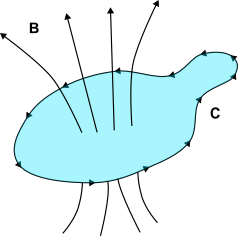
\includegraphics[width=0.32\textwidth]{images/faraday_law}
\end{wrapfigure}
Consideriamo un filo come un conduttore, avvolto attorno ad una curva stazionaria C. Un filo chiuso prende il nome di circuito. Se integriamo l'equazione (5.1) rispetto alla superficie S racchiusa dal circuito chiuso C, abbiamo che
\begin{equation*}
	\int_{S}(\nabla \times \bold{E}) \cdot d \bold{S} = - \int_{S} \frac{\partial \bold{B}}{\partial t} \cdot d\bold{S}
\end{equation*}
utilizzando il teorema di Stokes possiamo riscrivere l'equazione come
\begin{equation*}
	\oint_{C} \bold{E} \cdot d\bold{r} = - \int_{S} \frac{\partial \bold{B}}{\partial t} \cdot d \bold{S} = - \frac{d}{dt} \int_{S} \bold{B} \cdot d \bold{S}
\end{equation*}
Per ottenere l'ultima relazione abbiamo assunto che n\`e C e n\`e S possano cambiare nel tempo. L'integrale di linea attorno a C del campo elettrico prende il nome di \textit{forza elettromotrice}, $\mathcal{E}$, che di solito viene abbreviata con $fem$.
\begin{equation*}
	\mathcal{E} = \oint_{C} \bold{E} \cdot d \bold{r}
\end{equation*}
La forza elettromotrice non \`e realmente una forza come possiamo vedere dalla sua espressione, in realt\`a \`e la componente tangenziale della forza per unit\`a di carica, integrata lungo un filo. Un altro modo di vederla \`e dato dal lavoro necessario a spostare una carica unitaria lungo la curva C. Se la $fem$ \`e non nulla allora \`e presente della carica accelerata all'interno del filo che genera quindi una corrente.

L'integrale del campo magnetico passante attraverso la superficie S prende il nome di flusso magnetico $\Phi$ attraverso la superficie S,
\begin{equation*}
	\Phi = \int_{S} \bold{B} \cdot d\bold{S}
\end{equation*} 
Di conseguenza possiamo riscrivere l'equazione di Maxwell (5.1) come 
\begin{equation}
	\mathcal{E} = - \frac{d\Phi}{dt}
\end{equation}
In questa forma l'equazione prende il nome di \textit{legge di Faraday}. 
\newline

\noindent La legge di Faraday ci dice che se cambiamo il flusso del campo magnetico attraverso una superficie S delimitata da un circuito, allora osserveremo un flusso di corrente all'interno del filo. Esistono diversi modi per modificare il campo magnetico, per esempio spostando una barra magnetica in vicinanza ad un circuito, passandola attraverso la superficie S delimitata dal filo conduttore. Un altro modo \`e dato muovendo un secondo filo $C''$ attraverso da una corrente, oppure tenendolo fisso e variando l'intensit\`a di corrente al suo interno accendendolo e spegnendolo. Tutti questi metodi inducono una corrente in C.
\newline

Esiste anche un secondo effetto, dovuto al fatto che dato un campo magnetico variabile e avendo una corrente indotta all'interno del circuito C, avremo che a sua volta la carica in moto genera un suo campo magnetico. Il campo magnetico indotto \`e orientato sempre in opposizione al cambiamento. Questo fenomeno prende il nome di \textit{legge di Lenz} e giustifica il segno negativo nella legge di Faraday (5.2). 

\subsection{Esempio legge di Lenz}

\begin{wrapfigure}{r}{0.4\textwidth} % 'r' for right, 'l' for left
    \centering
    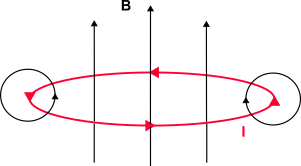
\includegraphics[width=0.38\textwidth]{images/lenz_law}
\end{wrapfigure}
Possiamo dimostrare la legge di Lenz con un semplice esempio. Consideriamo un caso in cui il cammino C \`e una circonferenza giacente in un piano, e ipotizziamo che sia immersa in campo magnetico B uniforme che al passare del tempo questo diventa pi\`u piccolo e dunque $\dot{\Phi} < 0$. Per la legge di Faraday abbiamo che $\mathcal{E} > 0 $ e la corrente scorre in senso antiorario lungo C. La corrente indotta genere una campo $\bold{B}$ che incrementa il campo all'interno della spira opponendosi alla sua decrescita.

\subsection{Esempio: generatori elettrici}


 